\documentclass[a4paper, 12pt]{article}
\usepackage[utf8]{inputenc}
\usepackage{geometry}
\usepackage{polski}
\usepackage{graphicx}
\usepackage{float}
\usepackage{etoolbox,refcount}
\usepackage{multicol}
\usepackage{tabularx}

\newgeometry{left=2cm, right=2cm, bottom=2cm, top=1.5cm}

\begin{document}
	\begin{figure}[H]
		\centering
		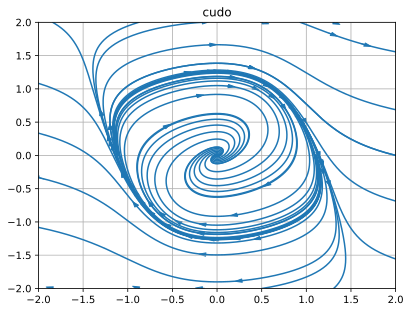
\includegraphics[width = \textwidth]{./img/cudo.png}
	\end{figure}
	\section{Cel ćwiczenia}
		Celem ćwiczenia jest zapoznanie się z zastosowaniem metody płaszczyzny fazowej do analizy nieliniowych układów regulacji na przykładzie serwomechanizmu przekaźnikowego. 
	\section{Wstęp}
		Układ posiada ujemne sprzężenie zwrotne, które jest podawane na układ dwóch przekaźników, których wyjścia są sumowane i podłączane pod bloczek strefy martwej. Takie połączenie bloczków przekaźników, sumatora i bloczka strefy martwej zachowuje się jako regulator trójpołożeniowy z histerezą.
		\begin{figure}[H]
			\centering
			\includegraphics[width = 0.8\textwidth]{./img/uklad.png}
			\caption{Schemat}
		\end{figure} \noindent
		Następnie mamy do czynienia z fragmentem układu, który ma przedstawiać obiekt o transmitancji $G(s) = \frac{K}{s(Ts+1)}$. Niestety nie jest to zgodne z prawdą, gdyż transmitancja takiego układu zadana jest wzorem:
		$$
			G(s) = \frac{K\cdot \frac{1}{s}}{1+\frac{T}{s}} \cdot \frac{1}{s} = \frac{K}{s(s+T)}
		$$
		Kontynuując ćwiczenie przyjęliśmy, że schemat blokowy jest poprawny, gdyż taki wariant pasował do podpunktu o podwójnym całkowaniu.
	\section{Wyniki}
		Poprzez automatyzację procesu przeprowadzenia symulacji (zagnieżdżone pętle for) udało nam się przeprowadzić na raz 2592 symulacji. Wykorzystaliśmy tym samym wszystkie możliwe kombinacje parametrów, jakie zostały nam podane w instrukcji. Jednak ze względu na czas jaki trwały same symulacje i konieczność dokonania ich jeszcze raz wraz z zapisem na dysk postanowiliśmy ograniczyć się do przypadków, które są wymagane w instrukcji.
		\subsection{Bez inercji, z histerezą}
			Parametry dobrane: $K = 1$, $T = 0$, $N = 0.1$, $h = 0.2$, $e_1 = 0$, $e_0 = 10$
			\begin{figure}[H]
				\centering
				\includegraphics[width = 0.85\textwidth]{./img/K_1_T_0_N_1_h_2_e1_0_e0_100.png}
			\end{figure} \noindent
			Po przebiegu trajektorii fazowej można wywnioskować, że odpowiedź czasowa będzie się rozbiegała (rosnący promień wodzący) oraz, że ma postać podobną do sinusoidy (pochodna jest przesunięta w stosunku do funkcji o kąt bliski prostemu i przeskalowana, tworząc figurę bliską elipsie). Brak inercji -- podwójne całkowanie -- sprawia, że układ się nie stabilizuje.
		\subsection{Z inercją, z histerezą}
			Parametry dobrane: $K = 1$, $T = 1$, $N = 0.1$, $h = 0.2$, $e_1 = 0$, $e_0 = 10$
			\begin{figure}[H]
				\centering
				\includegraphics[width = 0.85\textwidth]{./img/K_1_T_1_N_1_h_2_e1_0_e0_100.png}
			\end{figure} \noindent
			Po przebiegu trajektorii fazowej można wywnioskować, że odpowiedź czasowa jest sprowadzana w okolice zera, malejąc coraz szybciej. Następnie po przekroczeniu zera dochodzi do oscylacji wokół -- zataczane pętle na trajektorii fazowej.
		\subsection{Bez inercji, bez histerezy}
			Parametry dobrane: $K = 1$, $T = 0$, $N = 0.1$, $h = 0$, $e_1 = 0$, $e_0 = 10$
			\begin{figure}[H]
				\centering
				\includegraphics[width = 0.85\textwidth]{./img/K_1_T_0_N_1_h_0_e1_0_e0_100.png}
			\end{figure} \noindent
			Podobnie jak przedtem brak inercji uniemożliwia ustabilizowanie się układowi, brak histerezy natomiast nie pozwala na zwiększanie amplitudy. Po przebiegu trajektorii -- bliska kołowej -- można też wywnioskować, że odpowiedź czasowa będzie bliska sinusoidzie.
		\subsection{Z inercją, bez histerezy}
			Parametry dobrane: $K = 1$, $T = 1$, $N = 0.1$, $h = 0$, $e_1 = 0$, $e_0 = 10$
			\begin{figure}[H]
				\centering
				\includegraphics[width = 0.85\textwidth]{./img/K_1_T_1_N_1_h_0_e1_0_e0_100.png}
			\end{figure} \noindent
			Inercja oraz brak histerezy pozwala pozwala na stabilizację. Na przebiegu można zauważyć, że odpowiedź czasowa będzie miała najpierw dużą amplitudę, która będzie coraz szybciej malała, aż osiągnie wartość bliską zeru. Następnie szybko nastąpią szybko wytłumione oscylacje i układ będzie zmierzał do zerowego położenia i spoczynku.
	\section{Wnioski}
		Ćwiczenie te pozwoliło nam na zapoznanie się z nieliniowymi układami regulacji oraz z zastosowaniem płaszczyzny fazowej. Dowiedzieliśmy się jak przy pomocy przekaźników, węzła sumacyjnego oraz bloczka martwej strefy stworzyć regulator trójpołożeniowy z histerezą.
		\newline
		\newline 
		Dowiedzieliśmy się jaki związek ma płaszczyzna fazowa z odpowiedzią czasową układu oraz jesteśmy w stanie na podstawie jej przebiegu wywnioskować informacje o przebiegu odpowiedzi czasowej.
		\newline
		\newline
		Jedyną trudnością na jaką natknęliśmy się przy automatyzacji symulacji był bloczek odpowiedzialny za rysowanie trajektorii fazowych. Musiał mieć na sztywno w chwili symulacji przypisane osie oraz nie pozwalał na eksportowanie danych do środowiska MATLAB. Dlatego też podłączyliśmy dodatkowy oscyloskop, którego jedynym zadaniem było zbieranie danych do środowiska MATLAB. Następnie wyrysowaliśmy na podstawie danych z obydwu oscyloskopów trajektorie fazowe. 
\end{document}